\documentclass[english, 12pt, letterpaper]{article}
\usepackage[letterpaper, margin=1in]{geometry}
\usepackage[utf8]{inputenc}

\title{Characterizing the genetic interactions of \KRAS{} variants}
\author{
    Joshua Cook\textsuperscript{1,2,3},
    Giorgio Melloni\textsuperscript{3}, 
    Peter J. Park\textsuperscript{3,4}, 
    Kevin Haigis\textsuperscript{1,5{*}}
}

\usepackage[T1]{fontenc}
\usepackage{babel}
\usepackage{amsmath}
\usepackage{graphicx}
\usepackage{fancyhdr}
\pagestyle{fancy}
\fancyhf{}
\renewcommand{\headrulewidth}{0pt}
\setlength{\headheight}{0pt}

% Supplemental figure numbering.
\newcommand{\beginsupplement}{%
        \setcounter{table}{0}
        \renewcommand{\thetable}{\arabic{table}}%
        \setcounter{figure}{0}
        \renewcommand{\thefigure}{\arabic{figure}}%
     }

% Single spaces after periods.
\frenchspacing

% Page numbering.
\pagenumbering{arabic}
\rfoot{\thepage}

% Font to Helvetica.
\usepackage{helvet}
\renewcommand{\familydefault}{\sfdefault}

% Specific command for the KRAS gene.
\newcommand{\KRAS}{\emph{KRAS}}
% Specific command for the KRAS protein.
\newcommand{\kras}{KRas}

\begin{document}

\maketitle

\thispagestyle{fancy}

1. Cancer Research Institute, Beth Israel Deaconess Medical Center, Boston, Massachusetts.
2. Department of Medicine, Harvard Medical School, Boston, Massachusetts.
3. Department of Biomedical Informatics, Harvard Medical School, Boston, Massachusetts, USA.
4. Ludwig Center at Harvard, Boston, MA 02115, USA.
5. Harvard Digestive Disease Center, Harvard Medical School, Boston, Massachusetts.

{*}corresponding author(s):
Kevin M Haigis (khaigis@bidmc.harvard.edu)

\begin{abstract}
An activating mutation in the \KRAS{} gene is an initiating event in many cancers.
Though the mutant variants are seemingly similar, the biology of each is distinct and clinically relevant.
However, the broader effects on the genomic landscape during oncogenesis have yet to be explored.
To this end, 13,492 samples were collated from four tumor types with the highest frequency of mutation in \KRAS{}, colorectal adenocarcinoma (COAD), lung adenocarcinoma (LUAD), multiple myeloma (MM), and pancreatic adenocarcinoma (PAAD).
Investigating the origin of mutation revealed that most mutant alleles could not be predicted by the prevalence of known mutagens.
Further, distinct comutation networks were resolved for each allele.
 
\end{abstract}



\section*{Introduction}





\section*{Results}

\subsection*{\KRAS{} alleles are non-uniformly distributed across cancers.}

\KRAS{} was most frequently mutated at one of four “hotspots.” 
Of these hotspots, codon 12 mutations accounted for 81 \% of all mutations followed by codons 13 (8.4 \%), 61 (7.3 \%) and 146 (2.5 \%) (Fig. \ref{fig:mutational-signatures-main}a, Supplementary Fig. \ref{sfig:expanded-kras-allele-distribution}). 
Further, there was substantial variability of the alleles found at these hotspots across the \KRAS{}-driven cancers, COAD, LUAD, MM, and PAAD (Fig. \ref{fig:mutational-signatures-main}b). 
Notably, the most variation in \KRAS{} alleles was found in MM, and it is the only cancer where a non-G12 allele is the most frequent. 
COAD had a unique enrichment of G13D and A146T alleles while PAAD was unique in its high frequency of G12R mutations.


\subsection*{The \KRAS{}-alleles have different mutagenic origins.}

Most \KRAS{} mutations were caused by single nucleotide variants.
An exception was the exceedingly rare, though transformative in vitro \cite{Barbacid1987}, G12F allele (0.4 \%) caused by the dinucleotide substitution c.34\_35GG>TT. Glycine 12 and 13 can be transformed to six different amino acids (C, D, S, R, A, and V) through single nucleotide changes in the first two cytosines.
Glutamine 61 can mutate to only four other amino acids (H, K, L, and R).

The active mutational processes in the tumor samples were elucidated using mutational signatures \cite{Alexandrov2013}. 
Briefly, all single-nucleotide mutations can be represented by the combination of the six possible pyrimidine to purine base substitutions (C>T, C>A, C>G, T>A, T>C, T>G) and all possible 3’ and 5’ flanking bases. 
This composes a mutational spectrum with 96 possible trinucleotide contexts. 
The signatures were discovered using non-negative matrix factorization and measured in each sample using non-negative least squares regression (see methods for the complete details). 

The distribution of the levels of each mutational signature were generally uniform within a cancer, regardless of the \KRAS{} allele of the tumor (Supplementary Fig. \ref{sfig:mutational-signatures-summary}a, b, c). 
An apparent exception was for microsatellite instable (MSI) tumors, where the signatures associated with that characteristic dominated (these samples were not included in Fig. \ref{fig:mutational-signatures-main} nor Supplementary Fig. \ref{sfig:mutational-signatures-summary}c). 
For each tumor with a \KRAS{} mutation, the probability that the allele was caused by each detectable mutational processes was calculated. 
The average of these probabilities for each allele were shown in Fig. \ref{fig:mutational-signatures-main}c. 
Most of the common \KRAS{} mutations in COAD, MM, and PAAD, were likely caused by mutations in “clock-like” signatures 1 and 5, mutations believed to accumulate with age \cite{Alexandrov2015} (Supplementary Fig. \ref{sfig:mutational-signatures-summary}b). 
LUAD was the only cancer with \KRAS{}-mutant samples enriched for a mutational signature of exogenous cause. 
Samples with \KRAS{} G12A/C/V and G13C mutations were primarily burdened with mutations attributable to tobacco smoke (signature 4 \cite{Alexandrov2016}) while \KRAS{} G12D samples were split into about 25 \% signature 4 and about 75 \% signature 1 and 5 (Fig. \ref{fig:mutational-signatures-main}c, d).
Signature 8, of unknown etiology, had a substantial probability of causing some of the \KRAS{} alleles across all four cancers.

There were some interesting links between specific alleles and mutational signatures.
In COAD and PAAD, signature 18, likely caused by erroneous base excision repair of damage caused by reactive oxygen species \cite{Viel2017, Pilati2017}, was highly associated with G12C mutations (Fig. \ref{fig:mutational-signatures-main}c, d). 
This corroborated the previous finding that the \KRAS{} G12C mutation was more frequent in patients with MUTYH-Associated Polyposis \cite{Viel2017}, a recessive autosomal disease with increased risk for colorectal cancer. 
In MM, signature 9, associated with mutations introduced by polymerase $\eta$ linked to activation-induced deaminase (AID) \cite{Pavri2010Activation-inducedSpt5}, was strongly linked with Q61H (Fig. \ref{fig:mutational-signatures-main}c, d), the most common \KRAS{} mutation in the cancer.

Overall, with the exceptions noted above, most of the \KRAS{} alleles cannot be attributed to a unique mutational signature. 
Instead, they are primarily attributable to the most common mutational process in the tumors: age-related mutation in COAD, MM, and PAAD, and tobacco smoke in LUAD.


\subsection*{The frequency of most \KRAS{} alleles cannot be attributed to the prevalence of detected mutagens.}

The explanatory value of the mutational signatures was further analyzed by calculating the predicted frequency of each allele based on the frequency of mutations in the same trinucleotide context throughout the genome (Fig. \ref{fig:mutational-signatures-main}e, f).
The first null hypothesis tested was that, assuming the patient would acquire a \KRAS{} mutation, any of the common alleles were sufficient. Thus the frequency of the \KRAS{} alleles would be determined by the mutational processes, alone (Fig. \ref{fig:mutational-signatures-main}e).
The second null hypothesis was similar, but restricted to just codon 12 mutants (Fig. \ref{fig:mutational-signatures-main}f).
The predicted frequencies were compared against the observed allele frequencies.
The alleles above the diagonal line were predicted to be more frequent that actually observed, while those below the line were more frequent than predicted by the mutational signatures.
In LUAD and MM, most of the frequencies were predicted in the correct order, though the frequencies were significantly different in most cases (binomial test, p < 0.05, circles); this is especially apparent in MM when only considering the codon 12 mutants.
In COAD, G13D was predicted to be the most frequent allele, and G12D/V mutations were considerably underestimated.
However, if only codon 12 mutants were considered, the null hypothesis could not be rejected for G12D and G12V.
Importantly, the predictions have large confidence intervals suggesting a high amount of variation in the samples.
Inversely, the frequencies of A146T and G12S mutations were highly overestimated.
In MM, the most frequent allele, Q61H, was dramatically underestimated with a predicted frequency of 22 \% but actual frequency of 45 \% of \KRAS{} mutations.
In PAAD, all of the alleles were observed at a significantly different frequency than predicted by mutational signatures for both null hypotheses.
Thus, while it was likely that the active mutational processes in a tissue contributed to determining which \KRAS{} mutation was gained, they were unlikely to be deterministic.
This suggested that the particular properties of the alleles drive their selection, warranting further investigation into their genetic interactions.


\subsection*{The \KRAS{} alleles have distinct comutation networks.}

The \KRAS{} alleles can be further characterized by the genes they tend to comutate with.
An increased frequency of comutation suggests a synergistic effect whereas a reduced frequency of comutation suggests an inhibitory effect on growth, likely through a mechanism of collateral lethality.
The extreme of the latter effect is commonly known as "mutual exclusivity."
For instance, in COAD, \emph{APC} comutation enhances the effects of oncogenic \KRAS{}-induced hyperactivation of the Wnt signaling pathway, essential for the growth of cancer stem cells in the intestinal crypts \cite{Janssen2006, Fearon2014, Sakai2018, Jauhri2017}.
Alternatively, the activation of \emph{BRAF} via a V600E mutation was demonstrated to induce senescence in the presence of a \KRAS{} mutant, and, thus, the two are rarely found in the same tumor \cite{Seth2009ConcomitantCancer., Cisowski2016, Jauhri2017}.
The comutation network of each \KRAS{} allele for each cancer was constructed using a one-sided Fisher's exact test to detect genes with increased comutation and the Row Column test for Exclusivity to detect genes with reduced comutation \cite{Leiserson2016}.
The result of the analysis on COAD tumors was a weakly connected network of the \KRAS{} alleles with only a few genes linking the alleles together (Fig. \ref{fig:coad-comutation-main}a).
These linking genes tended to be well-known oncogenes such as \emph{BRAF}, \emph{APC}, and \emph{TP53}.
Contrary to common assumption, while \KRAS{} and \emph{TP53} are frequently found mutated in the same tumor, there is a detectable reduction in comutation of \emph{TP53} with \KRAS{} G12D and G13D (Fig. \ref{fig:coad-comutation-main}a, b).

Surprisingly, there were a substantial number of genes detected to comutate with just one \KRAS{} allele.
To gain functional insight into the network, genes known to physically interact with \KRAS{} \cite{Kovalski2019}, signal up- or downstream of \KRAS{} \cite{Kanehisa2017, Kanehisa2016KEGGAnnotation.}, or are known oncogenes \cite{Bamford2004TheWebsite., Sondka2018} were extracted (Fig. \ref{fig:coad-comutation-main}b).
As expected, several alleles had reduced comutation with \emph{NRAS} and \emph{BRAF} and increased comutation with \emph{APC} and \emph{PIK3CA}. Some novel interactions included increased comutation of \emph{PORCN} with \KRAS{} A146T, \emph{MTOR} with G12C, and \emph{SMAD4} with G12V.
Further, several of the alleles showed enrichment for cellular functions in their comutation networks (Fig. \ref{fig:coad-comutation-main}c).
One of the strongest effects was an enrichment in the G12D comutation network of interactors with \emph{YWHAZ}, a 14-3-3 scaffolding protein implicated in modulating many interactions including Arhgef7 activity on Rac1 \cite{Angrand2006TransgenicSignaling.}.
Also, genes involved in the Hippo and Wnt signaling, key pathways in COAD, were enriched in the comutation networks of \KRAS{} G12V and G13D.

% I didn't reference Fig. 2 e-g because there wasn't anything specific to say about them, and there is not enough space to expand upon them for each cancer. They are explained in the legend and are just an interesting visualization of comutation interactions.












\section*{Discussion}





\section*{Methods}

\subsection*{Data sources and acquisition}

Whole genome sequencing (WGS), whole exome sequencing (WXS), and targeted gene panel sequencing data were collected of colorectal adenocarcinoma (COAD), lung adenocarcinoma (LUAD), multiple myeloma (MM), and pancreatic adenocarcinoma (PAAD).
WXS and WGS data were downloaded from cBioportal \cite{Gao2013, Cerami2012}, which included relevant project from The Cancer Genome Atlas (TCGA) \cite{CancerGenomeAtlasNetwork2012, CancerGenomeAtlasResearchNetwork2014, CancerGenomeAtlasResearchNetwork.Electronicaddress:andrew_aguirredfci.harvard.edu2017} and other smaller studies. 
Additional data were acquired from the International Cancer Genome Consortium (ICGC) for pancreatic cancer \cite{Scarlett2011} and colorectal cancer. 
Panel data for multiple cancers were retrieved from the Genomics Evidence Neoplasia Information Exchange (GENIE) consortium \cite{AACRProjectGENIEConsortium2017AACRConsortium.}.
GENIE data are an aggregation of several different panels ranging from ~30 genes to ~600.
\KRAS{} was included in all of the libraries. 
A detailed list of all cancer studies can be found in Supplementary Table 1.


\subsection*{Hypermutated sample cutoff}

Some of the COAD samples had 5 to 10-times more mutations than average, often due to microsatellite instability (MSI). 
A Gaussian mixed model was used to find the optimal cutoff based on available WGS and WXS data (Supplementary Fig. X). 
The top 17 \% and 21 \% of samples were considered hypermutants in WGS and WXS, respectively.
The same 17 \% cutoff was applied to the gene panel data. 
Hypermutants were not excluded from the identification of mutational signatures as they signature 6 is caused by MSI.
Samples with less than 40 mutations were removed.


\subsection*{Tissue gene expression filter}

A conservative filter of tissue-specific gene expression was used to remove genes not expressed in the tissues of study. 
Normal tissue gene expression data was gathered from the GTEx Portal (12/03/2018) \cite{GTExConsortium2017} and The Human Protein Atlas (HPA, 12/03/2018) \cite{Uhlen2015, Uhlen2016}, and tumor expression data was collected from MMRF-CoMMpass (01/14/2019), TCGA-COAD, TCGA-LUAD, and TCGA-PAAD \cite{CancerGenomeAtlasNetwork2012, CancerGenomeAtlasResearchNetwork2014, CancerGenomeAtlasResearchNetwork.Electronicaddress:andrew_aguirredfci.harvard.edu2017}. 
Supplementary Table 2 indicates the number of samples per tissue in the GTEx and tumor gene expression data. 
A gene was considered “expressed” in a tissue if it met at least one of the following criteria: 1) a median expression level of at least 1 TPM across all samples of the tissue in GTEx, 2) indicated as expressed at at least 1 TPM in the HPA data set for the tissue, 3) expressed with a median level of 1 RESM in the corresponding tumor RNA-sequencing data.
Supplementary Fig \ref{sfig:mutfreq-of-unexpressed-genes} indicates the frequency of mutation of genes that were removed from each tumor type according to this filter.


\subsection*{Identifying mutational signatures}

The genome-wide mutations of a sample can be deconvolved into mutational signatures that represent endogenous or exogenous mutagenic processes \cite{Alexandrov2013}. 
Single nucleotide variants (SNVs) from exomes or genomes were divided into 96 types, according to the 6 mutations of a pyrimidine (C>A, C>G, C>T and T>A, T>C, T>G) and the 16 possible combinations of 3’ and 5’ adjacent bases.
The MATLAB implementation of Non-Negative Matrix Factorization (NMF) algorithm, SigProfiler \cite{Alexandrov2013}, was used to discover the underlying mutational patterns that are common across tumors. 
Mutational signatures were discovered separately for each tumor type and the optimal number of signatures was determined based on silhouette width and frobenius error. 

The spectrum of the signatures discovered by NMF were matched to the COSMIC catalog \cite{Tate2019}.
For the signatures for which none of the 30 signatures in COSMIC catalog was found to be compatible, we referred to more recent studies in literature and expanded upon the COSMIC catalog. 
In particular, there were multiple subtypes of signature 7 (reported previously in \cite{Hayward2017Whole-genomeSubtypes., Alexandrov2018TheCancer}.
Further, the analysis revealed a signature that was dominantly C>A but not a subtype of signature 7.
This signature 38 was previously reported to be caused by indirect UV exposure \cite{Alexandrov2018TheCancer}. 
Three versions of the signature associated to POLE mutations, signature 10, were discovered (previously reported in \cite{Alexandrov2018TheCancer}.
These three POLE signatures differed in the C>A, C>T or C>G parts of the mutational spectrum. 
In LUAD, a signature with mutations of type C[C>A]N and T[C>A]N attributable to 8-oxo-guanine \cite{Alexandrov2018TheCancer} was found. 
One signature that we discovered COAD did not have a good match in any specific signature in literature, although it resembled a signature previously reported to be caused by SBSA \cite{Lee-Six2019} and signatures 34 and 41 in reference \cite{Alexandrov2018TheCancer}. 
This signature was not adjusted to resemble those previously reported because the results from different studies were not in strong agreement.
This signature referred to as N did not contribute to \KRAS{} mutations.
Three of the signatures discovered via NMF were likely to be artifacts \cite{Costello2013DiscoveryPreparation.} and were removed from downstream analysis. 
Signatures present at very low levels were removed and the levels of each signature were recalculated using Non-Negative Least Squares (NNLS) \cite{Gulhan2019DetectingSamples.}.
The results of this calculation were shown in Supplementary Fig X. 


\subsection*{Probability of \KRAS{} mutations from mutational signatures}

For each sample harboring a \KRAS{} mutation, the probability of occurrence given the mutational signatures present was calculated by considering the weight of the base change among the 96 possibilities and the relative contribution of the signature to the mutations in the sample. 
Thus, the probability $p$ of a tumor sample $a$ acquiring the \KRAS{} mutation $k$ from signature $s$ from all signatures $S$ can be calculated using Eq. \ref{eq:kras_mutation_from_signature}.

\begin{equation}
\label{eq:kras_mutation_from_signature}
p_{k,s} = \frac{c_{s,a} w_{k,s}}{\sum_{s}^{S} c_{s,a} w_{k,s}}
\end{equation}
\begin{equation*}
    \text{where} 
    \begin{cases}
        c_{s,a} \text{ is the contribution of signature $s$ in sample $a$.} \\
        w_{k,s} \text{ is the weight of the mutation $k$ in signature $s$.}
    \end{cases}
\end{equation*}


\subsection*{Comutation with \KRAS{} alleles}

A one-tailed Fisher’s exact test of independence was used to identify increased frequency of comutation between \KRAS{} alleles and other mutated genes. Only comutation partners with at least three comutation events were considered. Further, only genes with a mutation frequency of at least 1 \% or a comutation frequency of at least 10 \% were considered. 

The Row-Column Test for Exclusivity (RC-test) was used to identify reduced frequency of comutation between \KRAS{} alleles and other mutated genes \cite{Leiserson2016}. 
This is a permutation-based test that finds the probability of observing the actual number of mutually exclusive events given than the number of time the genes is mutated in all samples is fixed and the number of mutations in each sample is fixed.
Thus, the test conditions on both the frequency of mutation of the gene and the mutational burden of the samples.
Only genes with a mutational frequency of at least 2 \% and 10 mutually exclusive events were considered.


\subsection*{Predicting \KRAS{} allele frequency by mutational signatures}

The mutational signatures are linear combinations of the 96-dimension spectrum of possible mutations (see "Identifying mutational signatures" above).
Thus, assuming the null hypothesis that the prevalence of active mutational processes alone determines the frequency of \KRAS{} alleles in a cancer, the predicted frequency of each \KRAS{} allele can be calculated as the frequency of the same mutation across the entire genome.
The 95 \% confidence intervals were bootstrapped \cite{R-boot}.


\subsection*{Code availability}

All code is available at (GitHub repo).
See the README for the organization of the code and how to run the analysis.
Python \cite{van1995python} and R \cite{Rlang} were used for most of the analyses.



\section*{Acknowledgements}

The Acknowledgements should contain text acknowledging non-author contributors.
Acknowledgements should be brief, and should not include thanks to anonymous referees and editors or effusive comments.
Grant or contribution numbers may be acknowledged.

% Statement required by the MMRF.
These data were generated as part of the Multiple Myeloma Research Foundation Personalized Medicine Initiative.

\section*{Author contributions}

Each author’s contribution to the work should be described briefly, on a separate line, in the Author Contributions section. 

\section*{Competing interests}

A competing interests statement is required for all papers accepted by and published in \emph{Scientific Data}. If there is no conflict of interest, a statement declaring this must still be included in the manuscript.


\bibliography{reference_files/references, reference_files/R_citations, reference_files/additional_citations}{}
\bibliographystyle{plain}


\begin{figure}[p]
\centering
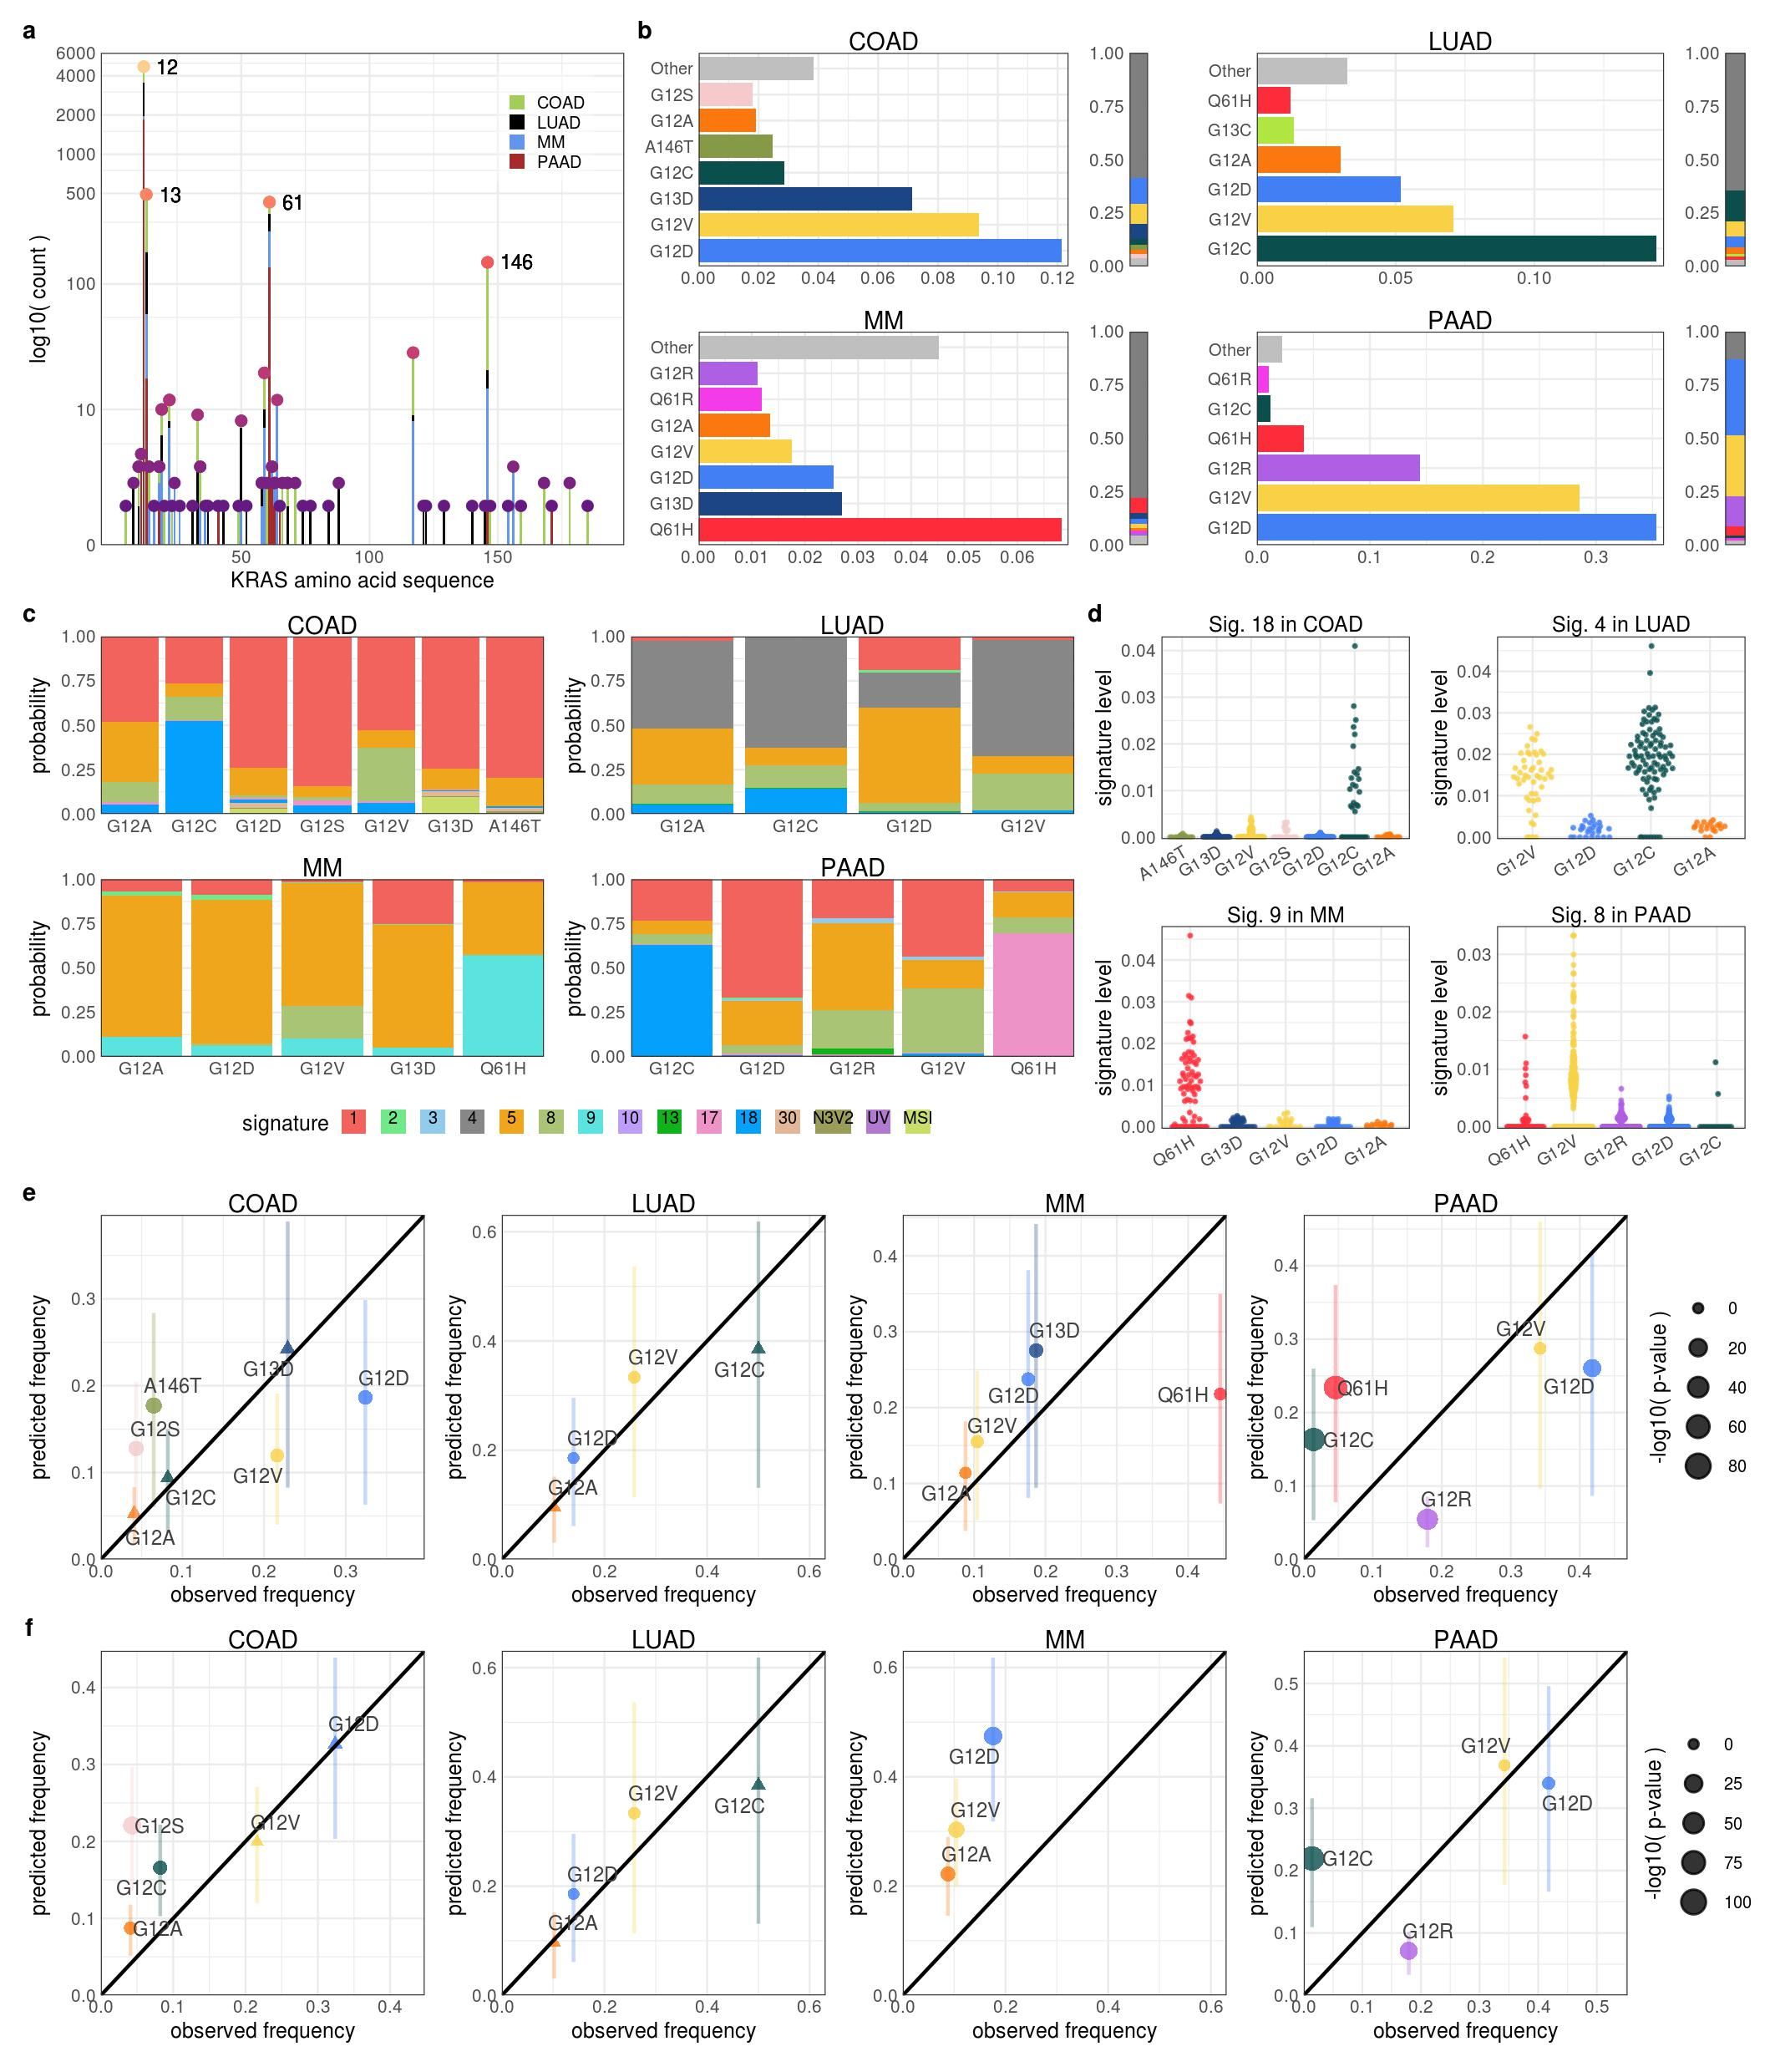
\includegraphics[height=160mm]{figures/Figure_01.jpeg}
\caption{
    \textbf{The levels of mutational processes do not explain the frequency of \KRAS{} alleles.}
    \textbf{a.} The number of samples with mutations along the \KRAS{} protein sequence. The most frequently mutated locations are labeled. The color of the bar indicates the abundance per cancer. 
    \textbf{b.} The distribution of \KRAS{} alleles in each cancer. The "Other" group includes the in-frequent \KRAS{} alleles. The adjacent bar indicates the fraction of samples with each \KRAS{} allele over all samples, including those with WT \KRAS{}.
    \textbf{c.} The average probability for each mutational signature causing the \KRAS{} mutant allele in a sample.
    \textbf{d.} The levels of select mutational signatures in samples with \KRAS{} mutations.
    \textbf{e, f.} The predicted vs. observed frequency of \KRAS{} alleles for all common alleles (\textbf{e}) or only codon 12 alleles (\textbf{f}). Triangles indicate the failure to reject the null hypothesis that the observed and predicted frequencies are the same. Error bars indicate boostrapped 95 \% confidence intervals.
    }
    \label{fig:mutational-signatures-main}
\end{figure}

\begin{figure}[p]
\centering
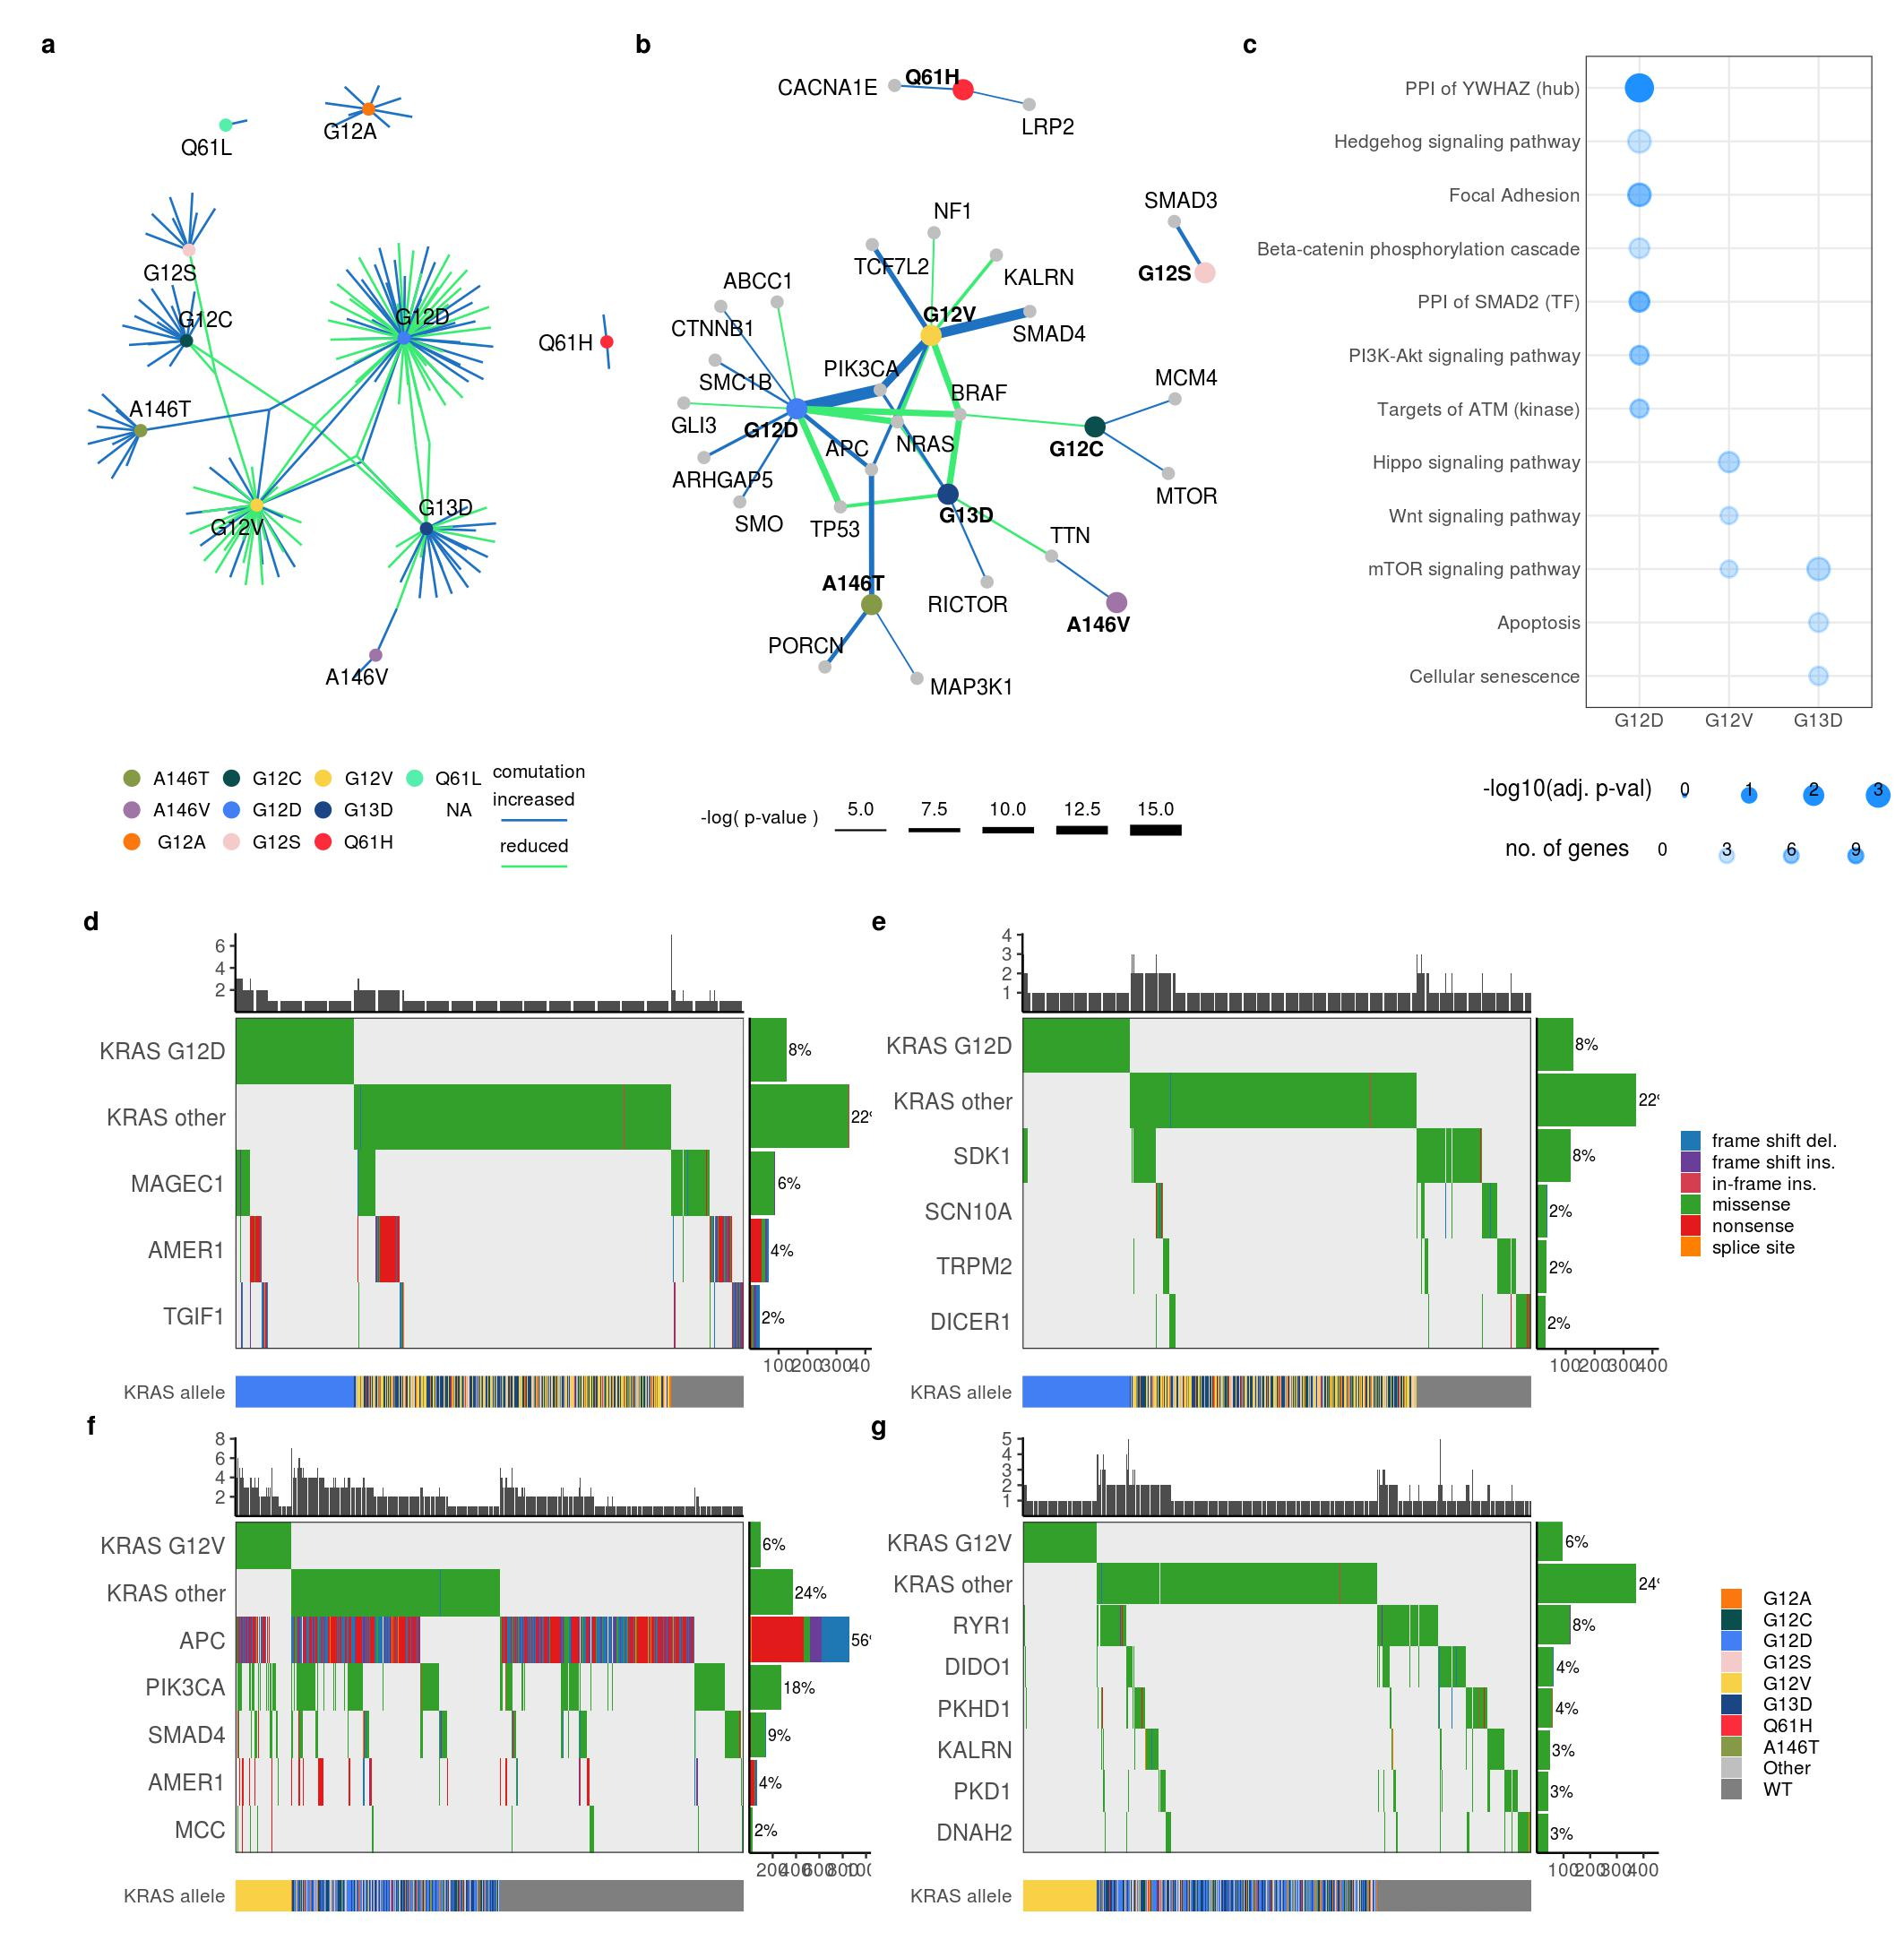
\includegraphics[height=135mm]{figures/Figure_02.jpeg}
\caption{
    \textbf{The comutation networks of common \KRAS{} alleles in COAD are distinct.}
    \textbf{a.} The comutation network of the \KRAS{} alleles in COAD with each edge representing a comutation interaction between an allele and another gene. The color of the edge indicates that the interaction was an increase (blue) or decrease (green) in the frequency of comutation.
    \textbf{b.} A subset of the network shown in \textbf{a} of genes known to physically interact with \KRAS{} or one of its canonical up- or downstream pathways. The width of the edge indicates the strength of the association.
    \textbf{c.} Cellular functions enriched in the comutation networks of the \KRAS{} alleles. The size of the dot indicates the strength of the association and the transparency indicates the number of genes in both the function and the comutation network.
    \textbf{d, e, f, g.} A visualization of the increased (\textbf{d}) or (\textbf{e}) decreased comutation of select genes with \KRAS{} G12D (\textbf{d, e}) and G12V (\textbf{f, g}). Rows of the central plot represent genes. Each column of the central plot is a different tumor sample. A filled space denotes a mutation of the gene in the sample, the color describing the type of variant. The bar plots above and to the right indicate the marginal values of the central plot. The row below the central plot indicates the \KRAS{} alleles of the tumor samples in the central plot.
}
\label{fig:coad-comutation-main}
\end{figure}

\begin{figure}
\centering
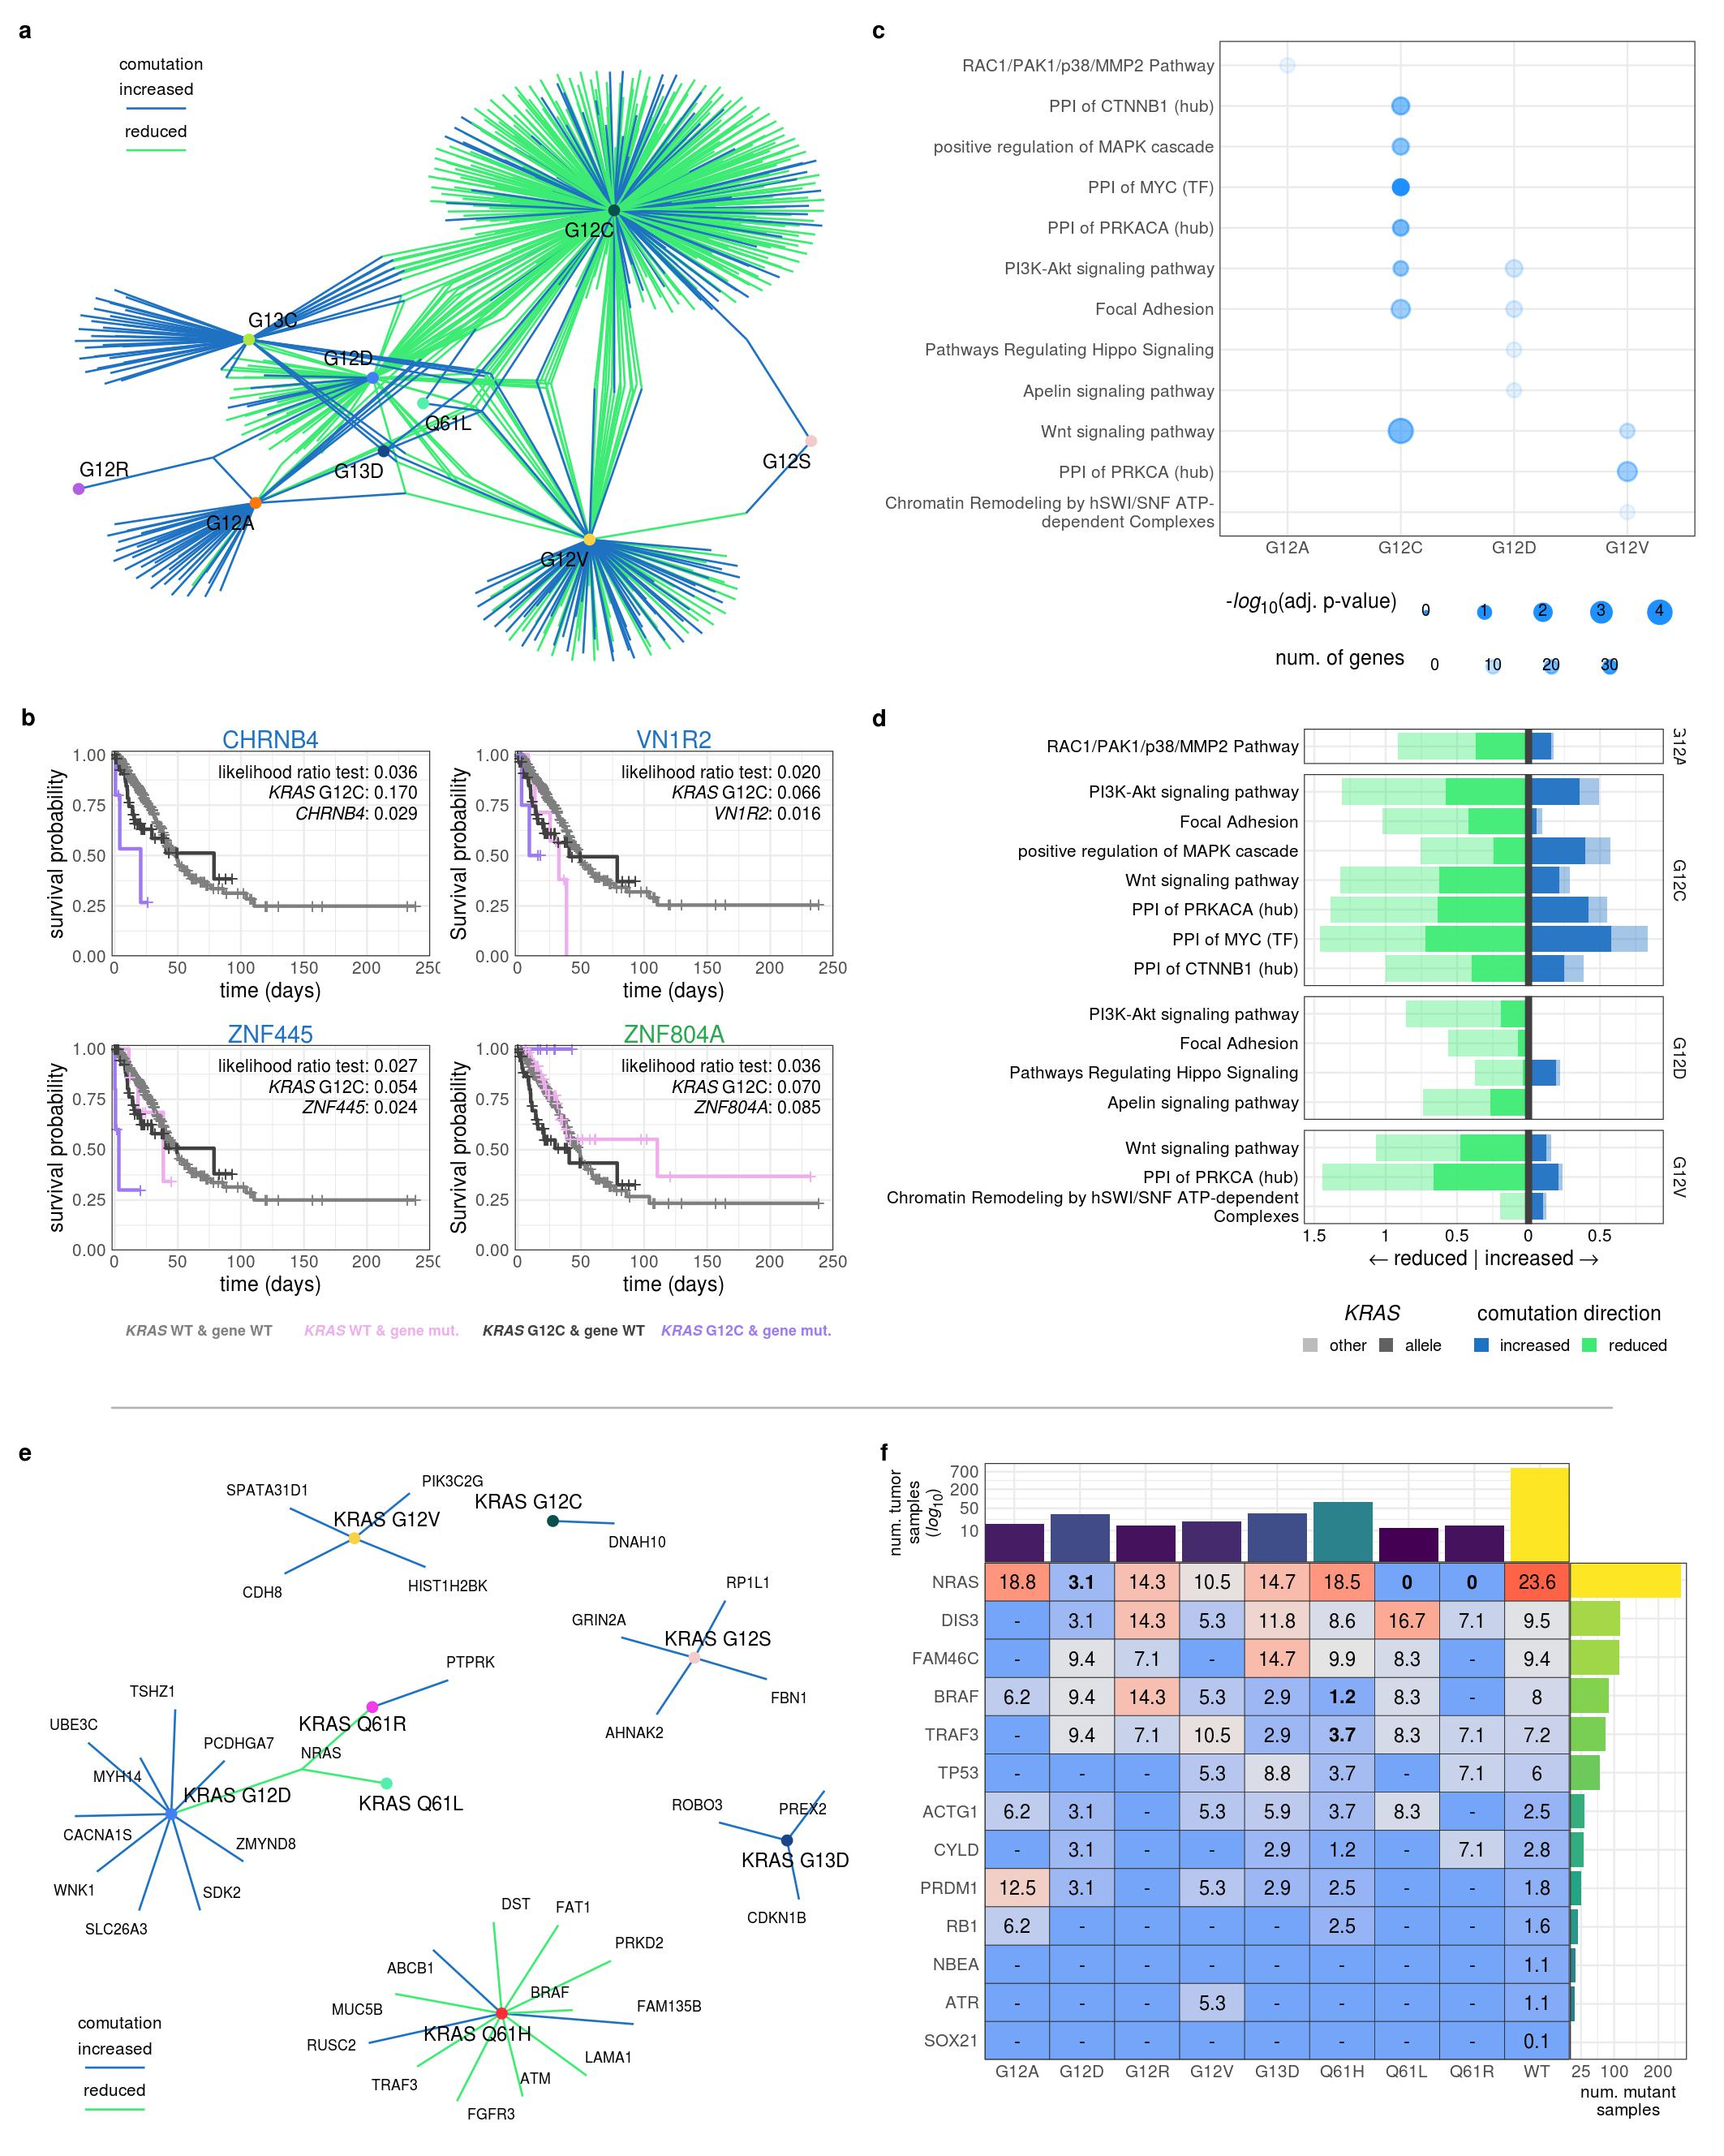
\includegraphics[height=150mm]{figures/Figure_03.jpeg}
\caption{
    \textbf{The comutation networks of \KRAS{} alleles in LUAD.}
    \textbf{a.} The comutation network of the \KRAS{} alleles in LUAD with each edge representing a comutation interaction between an allele and another gene. The color of the edge indicates that the interaction was an increase (blue) or decrease (green) in the frequency of comutation.
    \textbf{b.} Cellular functions enriched in the comutation networks of the \KRAS{} alleles. The size of the dot indicates the strength of the association and the transparency indicates the number of genes in both the function and the comutation network.
    \textbf{c.} The combined rate of comutation of the genes underlying the enriched functions shown in \textbf{b}. The x-axis indicates the rate at which one of the genes in the enriched function is mutated in the samples with the indicated \KRAS{} allele (dark) or the other samples (light). The genes were separated into those with an increase (blue, going right) or a reduced (green, going left) rate of comutation with the \KRAS{} allele.
}
\label{fig:luad-comutation-main}
\end{figure}


\beginsupplement

\begin{figure}[p]
\centering
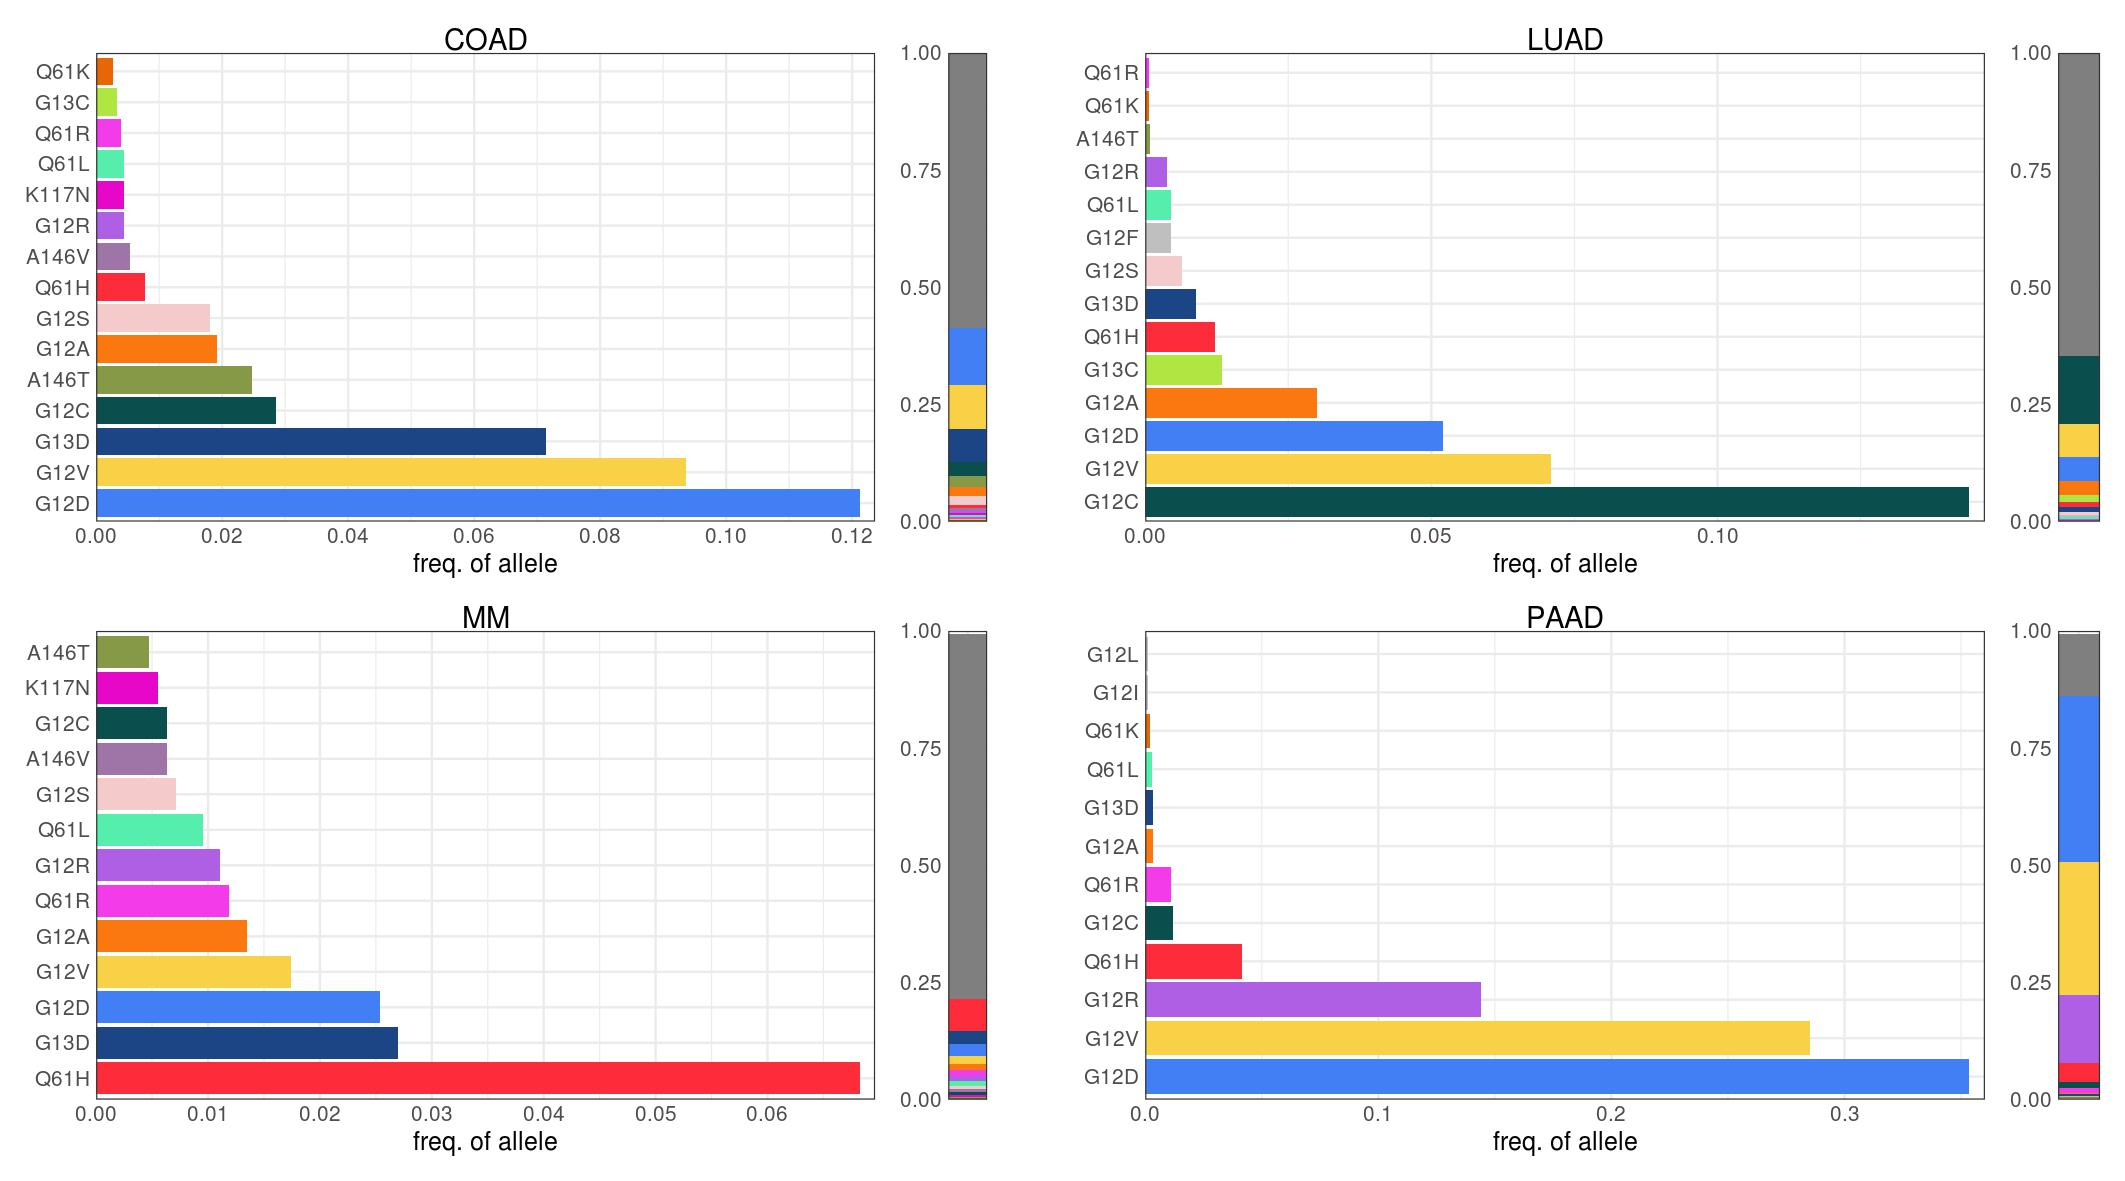
\includegraphics[width=\textwidth]{figures/SuppFigure_01.jpeg}
\caption{
    \textbf{The complete distribution of \KRAS{} alleles in each cancer.} The adjacent bar indicates the fraction of samples with each \KRAS{} allele over all samples, including those with WT \KRAS{}.
}
\label{sfig:expanded-kras-allele-distribution}
\end{figure}

\begin{figure}[p]
\centering
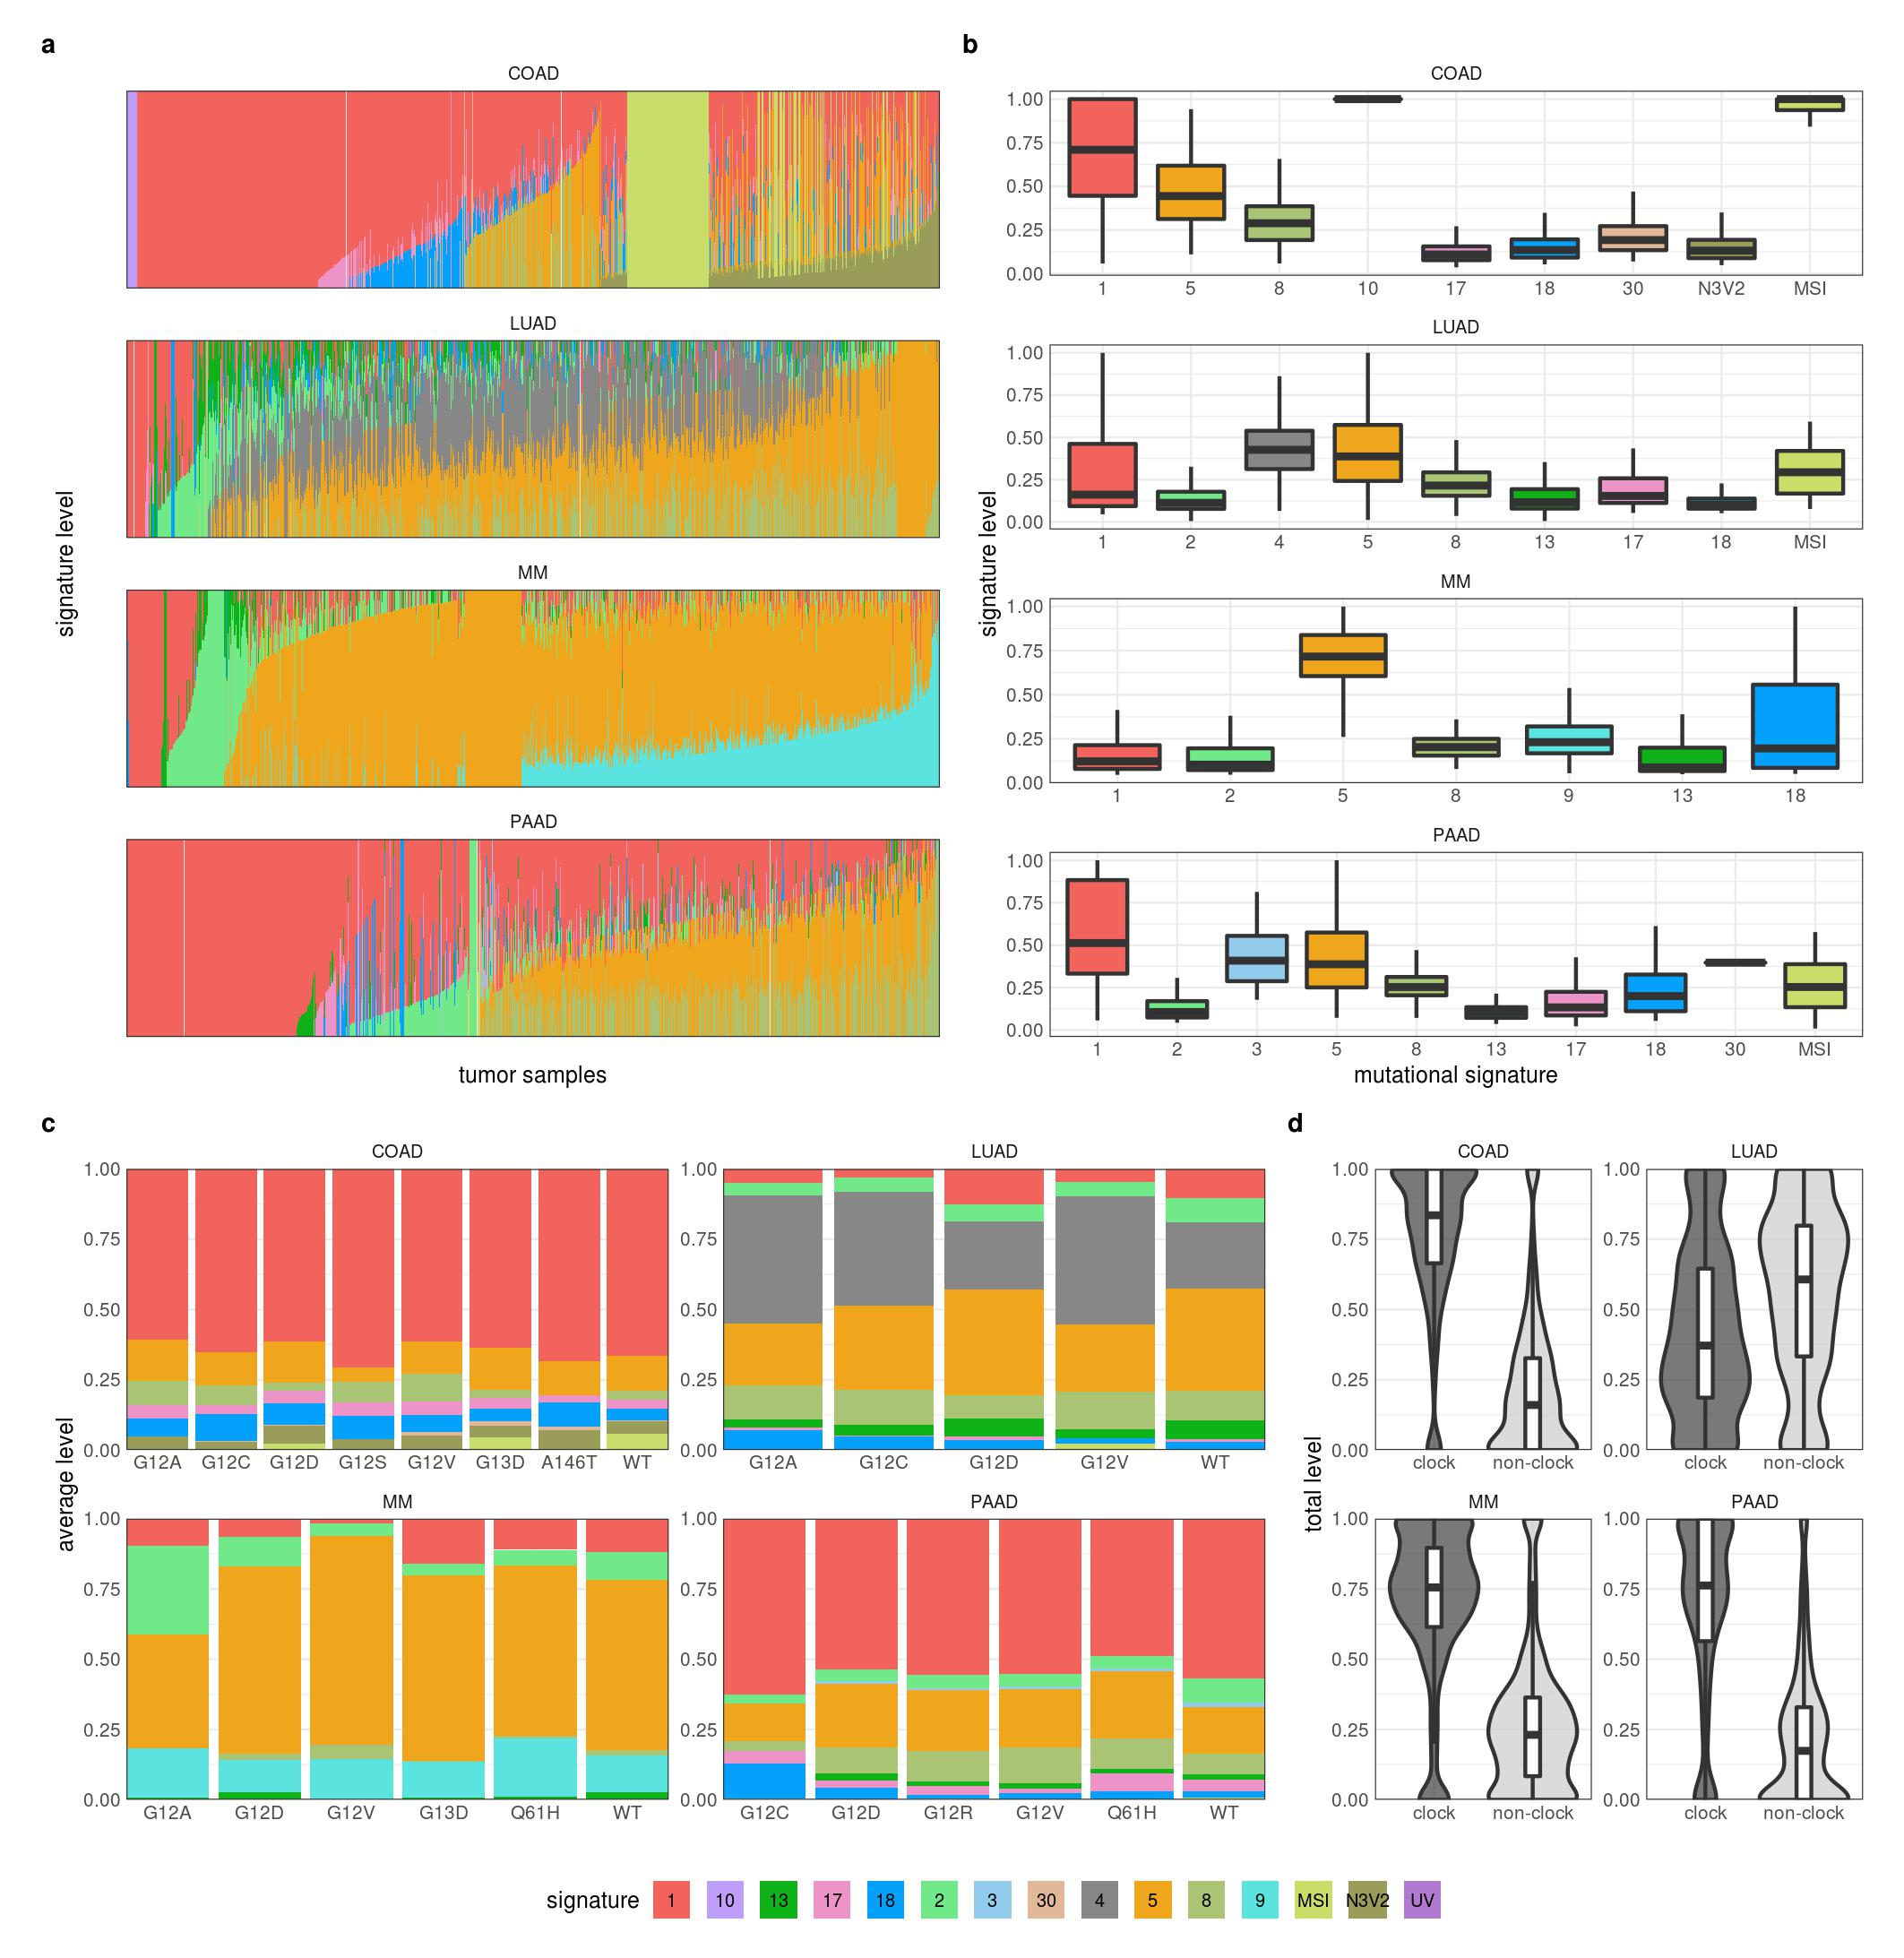
\includegraphics[height=160mm]{figures/SuppFigure_02.jpeg}
\caption{
    \textbf{Mutational signatures in tumor samples.}
    \textbf{a, b.} The detected level of the mutational signatures in each tumor sample.
    \textbf{c.} The average levels of mutational signatures in samples separated by \KRAS{} allele.
    \textbf{d.} The average levels of clock (signatures 1 and 5) and non-clock (all other signatures) in the tumor samples.
}
\label{sfig:mutational-signatures-summary}
\end{figure}

\begin{figure}[p]
\centering
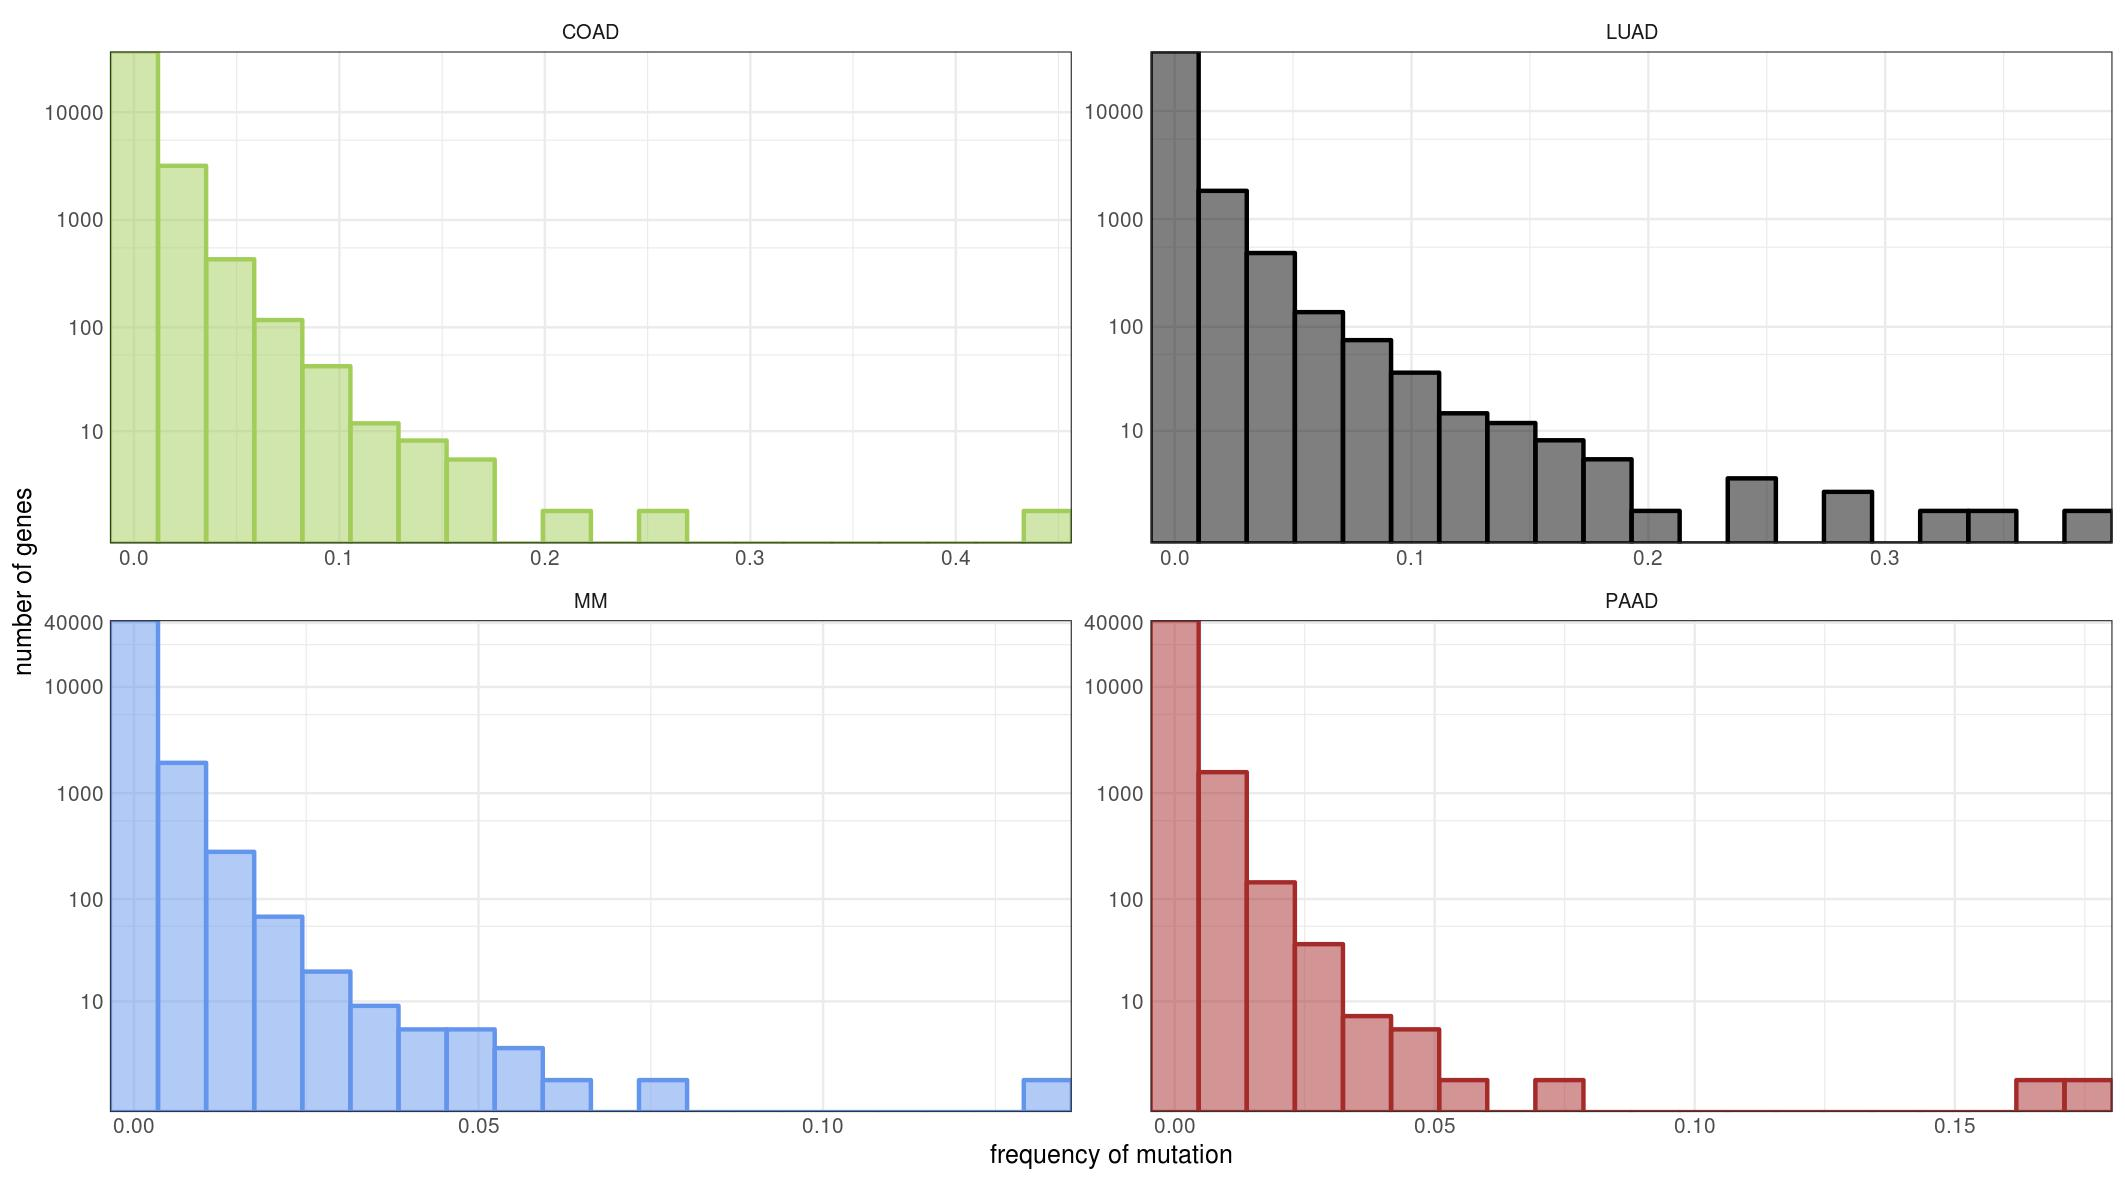
\includegraphics[width=\textwidth]{figures/SuppFigure_03.jpeg}
\caption{
    \textbf{The frequency of mutation of unexpressed genes.} Genes with no detectable level of expression in either cancer samples or normal tissue samples.
}
\label{sfig:mutfreq-of-unexpressed-genes}
\end{figure}


\end{document}
